\documentclass[twocolumn,
aps,
prx,
showpacs,
amsmath,
amssymb,
floatfix,
longbibliography,
superscriptaddress,
eprint]
{revtex4-1}

\usepackage{subfigure}
\usepackage{amsfonts} 

\usepackage{xcolor}
\definecolor{darkblue}{RGB}{0,0,150}
\definecolor{nightblue}{RGB}{0,0,100}

\usepackage{graphicx,mathtools,bm,bbm}
\usepackage{booktabs}
\usepackage{MnSymbol}
\usepackage[
colorlinks,
citecolor=darkblue,
linkcolor=darkblue,
urlcolor=nightblue]{hyperref}

\usepackage[english]{babel}
\usepackage[babel,kerning=true,spacing=true]{microtype}
\usepackage[utf8]{inputenc}

\usepackage{soul}

\newcommand{\ket}[1]{{\left|#1\right\rangle}}
\newcommand{\bra}[1]{{\left\langle #1\right|}}

\begin{document}

\title{Surface code ``off-the-hook''}
    
\author{Gilad Kishony}
\author{Austin Fowler}

\begin{abstract}
In the rotated surface code, hook errors---errors on auxiliary qubits midway through syndrome extraction that propagate to correlated two-qubit data errors---can reduce the circuit-level code distance by a factor of two if the extraction schedule is poorly chosen.
Traditional approaches use N-shaped and Z-shaped schedules, carefully selecting the orientation in each plaquette to avoid hook errors aligned with logical operators.
However, this strategy becomes increasingly complex for lattice surgery primitives with varied boundary geometries, and requires a 5-step schedule to avoid gate collisions.
We propose the diagonal schedule, which produces hook errors along the diagonal of each plaquette.
These diagonal errors trigger four stabilizers rather than two, making them non-matchable, and crucially never reduce the weight of any logical operator regardless of boundary orientation.
The diagonal schedule is globally uniform---all X-type plaquettes use one schedule and all Z-type plaquettes use another---eliminating the need for geometry-dependent planning.
On hardware supporting parallel measurement, reset, and gate operations, the schedule achieves a minimal period of 4 entangling gate time steps, compared to 5 for traditional approaches.
We demonstrate the diagonal schedule's effectiveness for memory experiments, spatial junctions, spatial Hadamard gates, and patch rotation, showing equivalent or improved logical error rates while simplifying circuit construction.
\end{abstract}
   
    
\maketitle

\section{Introduction}
\label{sec:intro}

The surface code is one of the leading candidates for fault-tolerant quantum computation due to its high threshold, local connectivity requirements, and compatibility with planar hardware architectures.
In the rotated surface code, quantum information is protected by measuring weight-4 stabilizer operators arranged on a square lattice, with X-type and Z-type stabilizers on alternating plaquettes.

A critical consideration in implementing the surface code is the design of the syndrome extraction circuit.
Each stabilizer measurement requires entangling an auxiliary qubit with the four data qubits of the plaquette through a sequence of two-qubit gates, followed by measurement of the auxiliary.
The order in which these gates are applied---the schedule---has profound implications for how errors propagate through the circuit.

A particularly problematic class of errors are hook errors: errors that occur on the auxiliary qubit midway through the syndrome extraction circuit.
Such an error propagates through the remaining two-qubit gates to become a correlated error on two data qubits.
The two affected data qubits are those that interact with the auxiliary in the second half of the circuit.
Critically, the Pauli type of the resulting two-qubit error matches the Pauli type of the stabilizer being measured.

If the syndrome extraction schedule is poorly designed, hook errors can reduce the effective code distance by a factor of two compared to the phenomenological noise case.
This occurs when hook errors create error chains that can propagate rapidly toward logical operators---paths between boundaries of the same Pauli type.

Traditional approaches to this problem use two schedule variants, commonly called N-shaped and Z-shaped schedules based on the pattern of gate ordering around the plaquette.
The N-shaped schedule produces vertical hook errors, while the Z-shaped schedule produces horizontal hook errors.
By carefully choosing between these schedules for each plaquette based on the boundary geometry, one can ensure that hook errors are oriented perpendicular to the problematic logical operator directions.

For a simple memory experiment with a single surface code patch---say, with X boundaries on the top and bottom and Z boundaries on the sides---the choice is straightforward: use Z-shaped schedules for X stabilizers (horizontal hooks) and N-shaped schedules for Z stabilizers (vertical hooks).
This ensures hook errors do not create short paths between same-type boundaries.

However, when performing computation using lattice surgery primitives, the situation becomes significantly more complex.
Lattice surgery operations create intricate three-dimensional spacetime geometries with boundaries of different Pauli types in various directions.
Planning which schedule to use in each plaquette to avoid all problematic hook errors becomes challenging and may be impossible in some configurations.
Furthermore, accommodating different N/Z schedules in adjacent regions requires a 5-step schedule to prevent collisions where two neighboring plaquettes would simultaneously apply gates to a shared data qubit.

An alternative approach to mitigating hook errors is to alternate the gate ordering between consecutive rounds of syndrome extraction~\cite{bluvstein2025architectural, gidney2024alternating}.
This approach offers a key advantage: one can use \emph{any} schedule uniformly across all plaquettes---even a ``bad'' choice that produces hook errors aligned with logical operators---and alternate between that schedule and its time-reversed version from round to round.
With this temporal alternation, only every other round has unfavorable hook error propagation, and the effective code distance becomes $d-1$ rather than the $\lfloor d/2 \rfloor$ that would result from using a fixed bad schedule.
However, sacrificing even a single unit of distance is a significant price to pay, especially for the small code distances relevant to near-term experiments where $d=3$ or $d=5$.
At $d=3$, for instance, an effective distance of 2 provides substantially less protection than distance 3.

\section{The Diagonal Schedule}
\label{sec:diagonal}

We propose the diagonal schedule as a solution to the limitations of traditional N/Z scheduling.
In the diagonal schedule, the four two-qubit gates of each stabilizer measurement are ordered such that the first two gates act on one diagonal pair of data qubits and the last two gates act on the opposite diagonal pair.

The key insight is that hook errors in this schedule affect two data qubits along the diagonal of the plaquette.
Unlike horizontal or vertical hook errors, diagonal errors have a fundamentally different relationship to the code's logical operators.

A diagonal hook error triggers four stabilizer measurements rather than two.
Consider an X-type hook error occurring in an X-stabilizer measurement: the two affected data qubits share edges with four neighboring Z-stabilizers, all of which will detect the error.
This makes diagonal hook errors non-matchable in the sense that they cannot be confused with lower-weight errors by a minimum-weight perfect matching decoder.

More importantly, diagonal hook errors never reduce the weight of any logical operator, regardless of the boundary geometry.
Logical operators in the surface code run between boundaries of the same type, following horizontal, vertical, or more complex paths depending on the patch shape.
A diagonal two-qubit error, being neither purely horizontal nor purely vertical, cannot create a shortcut along any of these paths.

The diagonal schedule offers several practical advantages:

\textbf{Global uniformity.}
All X-type plaquettes use the same schedule, and all Z-type plaquettes use the same schedule (related by Hadamard conjugation).
There is no need to analyze boundary geometries or plan schedule assignments---the same circuit works for any configuration.

\textbf{Reduced period.}
On hardware that allows measurement and reset operations to execute in parallel with unitary gates, the diagonal schedule achieves a period of 4 entangling gate time steps per syndrome measurement round.
Traditional N/Z scheduling requires 5 steps to avoid gate collisions between neighboring plaquettes with different schedules.

\textbf{Simplified circuit construction.}
The uniform nature of the diagonal schedule dramatically simplifies the construction of syndrome extraction circuits for complex lattice surgery operations.

The period of the diagonal schedule depends on hardware capabilities:
\begin{itemize}
    \item Period 7 if measurements and resets must occur in separate time steps from entangling gates
    \item Period 6 if no spatial Hadamard operations are required in a given time slice
    \item Period 4 if measurements, resets, and gates can all execute in parallel
\end{itemize}

\section{Memory Experiment}
\label{sec:memory}

We first demonstrate the diagonal schedule in the simplest setting: a memory experiment on a single surface code patch.
Figure~\ref{fig:memory} compares the traditional and diagonal schedules.

\begin{figure}
\centering
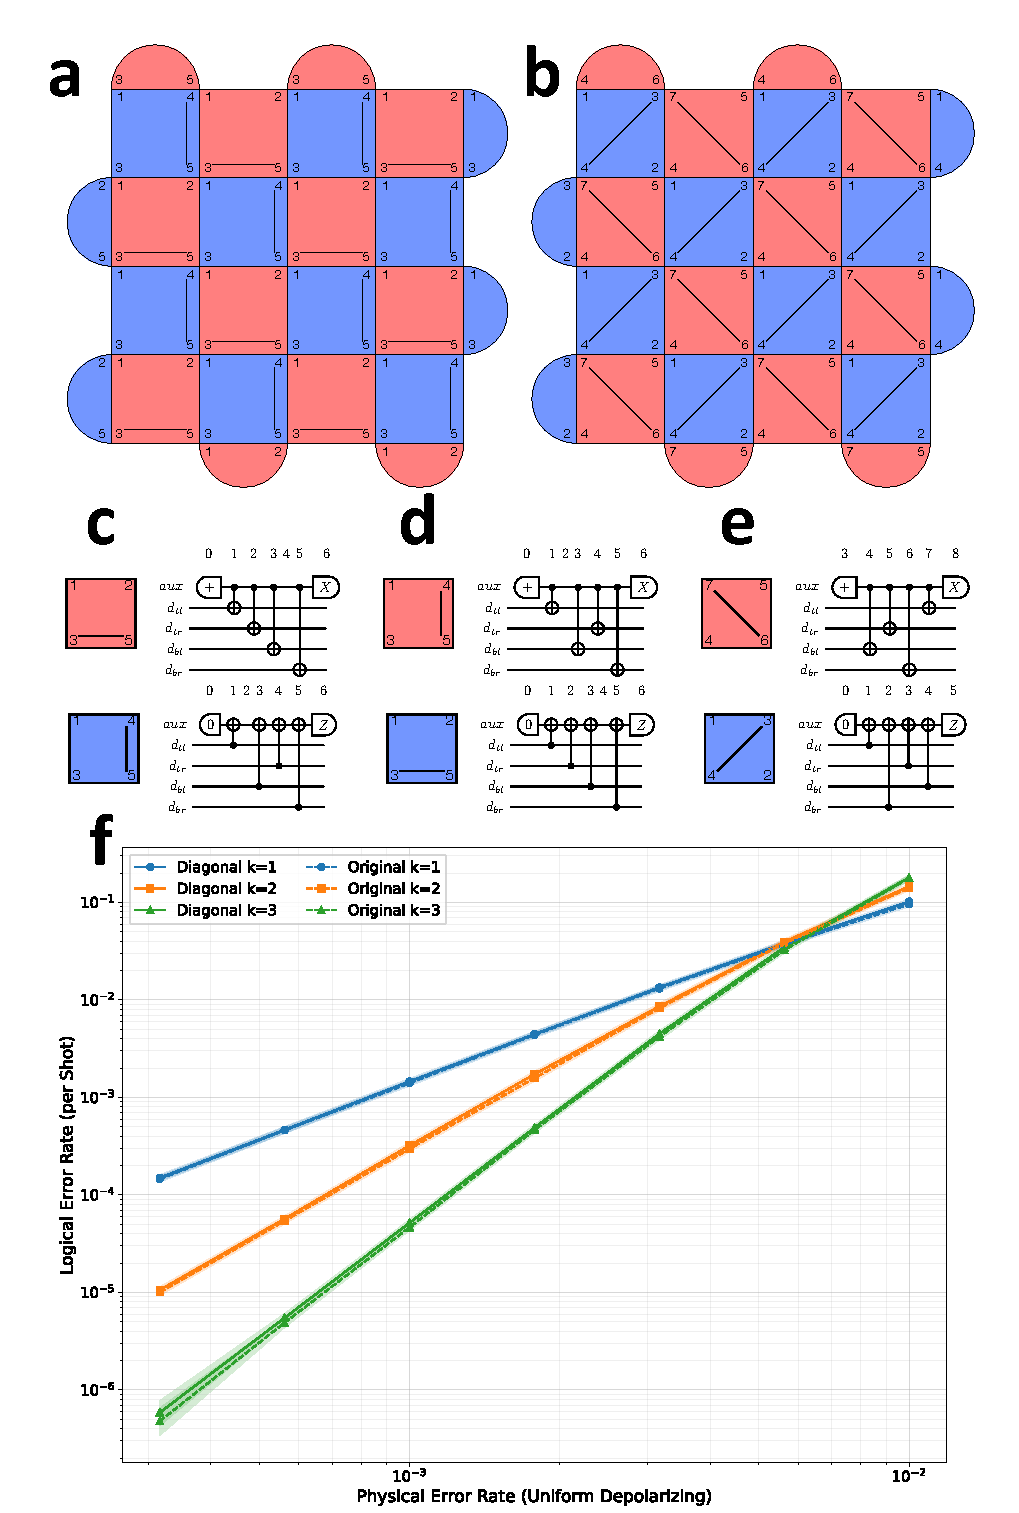
\includegraphics[width=\columnwidth]{memory.pdf}
\caption{
Memory experiment comparison.
\textbf{(a)} Standard N/Z schedule for a memory experiment, with schedule orientations chosen based on boundary types.
\textbf{(b)} Diagonal schedule for the same memory experiment, using a globally uniform schedule.
\textbf{(c)} Z-shaped X-plaquette and N-shaped Z-plaquette circuits with their corresponding schedule diagrams showing hook error orientations.
\textbf{(d)} Alternative orientation: N-shaped X-plaquette and Z-shaped Z-plaquette.
\textbf{(e)} Diagonal X-plaquette and Z-plaquette circuits with diagonal hook error orientations.
\textbf{(f)} Logical error rate versus physical error rate for standard (dashed) and diagonal (solid) schedules at various code distances $d = 2k+1$.
The two approaches achieve nearly identical logical error rates, demonstrating that the diagonal schedule preserves full code distance.
}
\label{fig:memory}
\end{figure}

Panels (a) and (b) show the plaquette layouts for standard and diagonal schedules respectively.
In the standard schedule, the orientation of each plaquette's gate ordering must be chosen based on the boundary geometry.
In the diagonal schedule, all plaquettes of the same type use identical circuits.

Panels (c) through (e) show the individual plaquette circuits and their corresponding hook error orientations.
The standard schedule produces horizontal hooks for Z-shaped plaquettes and vertical hooks for N-shaped plaquettes.
The diagonal schedule produces diagonal hooks that trigger four neighboring stabilizers.

Panel (f) presents benchmark results comparing logical error rates.
Both schedules are simulated with the same period-4 timing to isolate the effect of the schedule itself from timing differences.
The logical error rates are nearly identical across all code distances tested, confirming that the diagonal schedule preserves the full circuit-level code distance.

\section{Spatial Junctions}
\label{sec:junctions}

Lattice surgery operations require joining and splitting surface code patches, creating junction geometries where multiple boundaries meet.
These junctions present challenges for traditional scheduling because the optimal hook error orientation depends on which boundaries are active at any given time.

\subsection{L-Junction}

Figure~\ref{fig:l_junction} shows an L-shaped spatial junction where two patches meet at a corner.

\begin{figure}
\centering
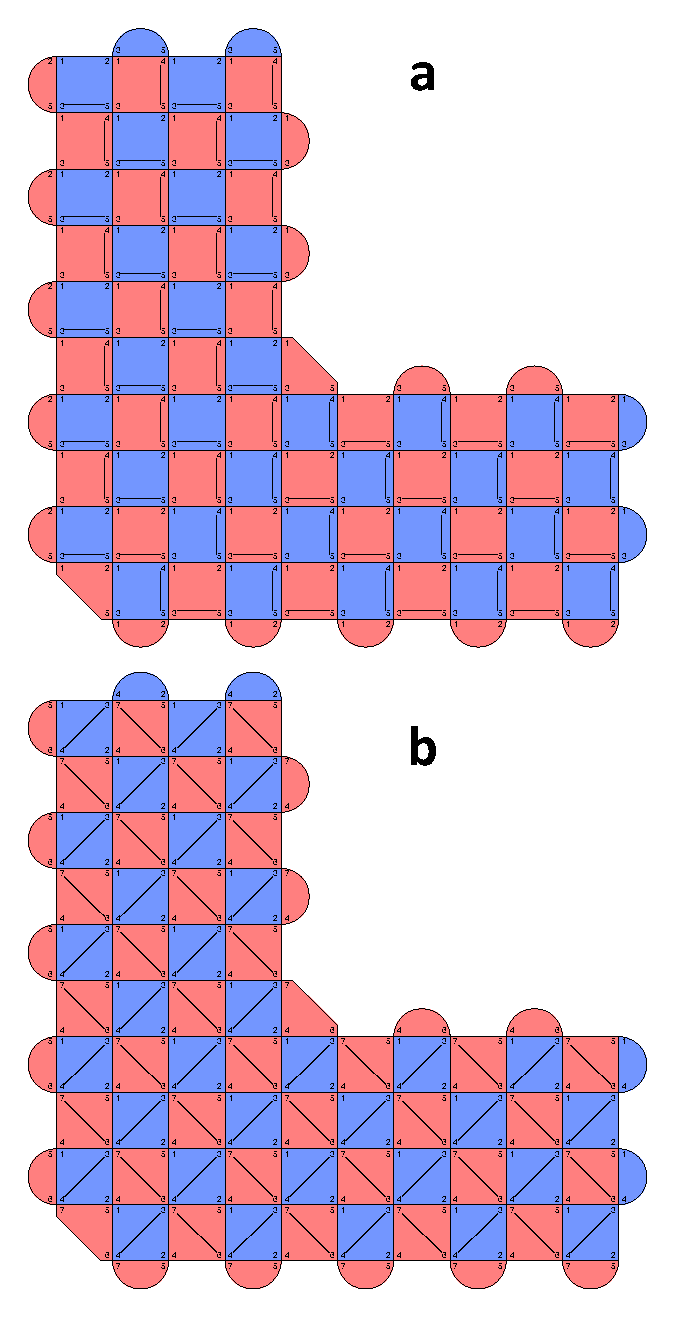
\includegraphics[width=\columnwidth]{L_junction.pdf}
\caption{
L-shaped spatial junction.
\textbf{(a)} Standard schedule with orientations chosen for the junction geometry.
\textbf{(b)} Diagonal schedule using the globally uniform circuit.
The diagonal schedule simplifies circuit construction while maintaining code distance.
}
\label{fig:l_junction}
\end{figure}

The L-junction demonstrates how the diagonal schedule eliminates the need to reason about which schedule orientations are appropriate at the junction.
With traditional scheduling, the plaquettes near the corner require careful analysis to avoid creating hook error paths that could reduce the effective distance.
The diagonal schedule simply uses the same circuit for all plaquettes, automatically avoiding problematic configurations.

\subsection{X-Junction}

Figure~\ref{fig:x_junction} shows an X-shaped junction where four patches meet, representing a more complex lattice surgery configuration.

\begin{figure}
\centering
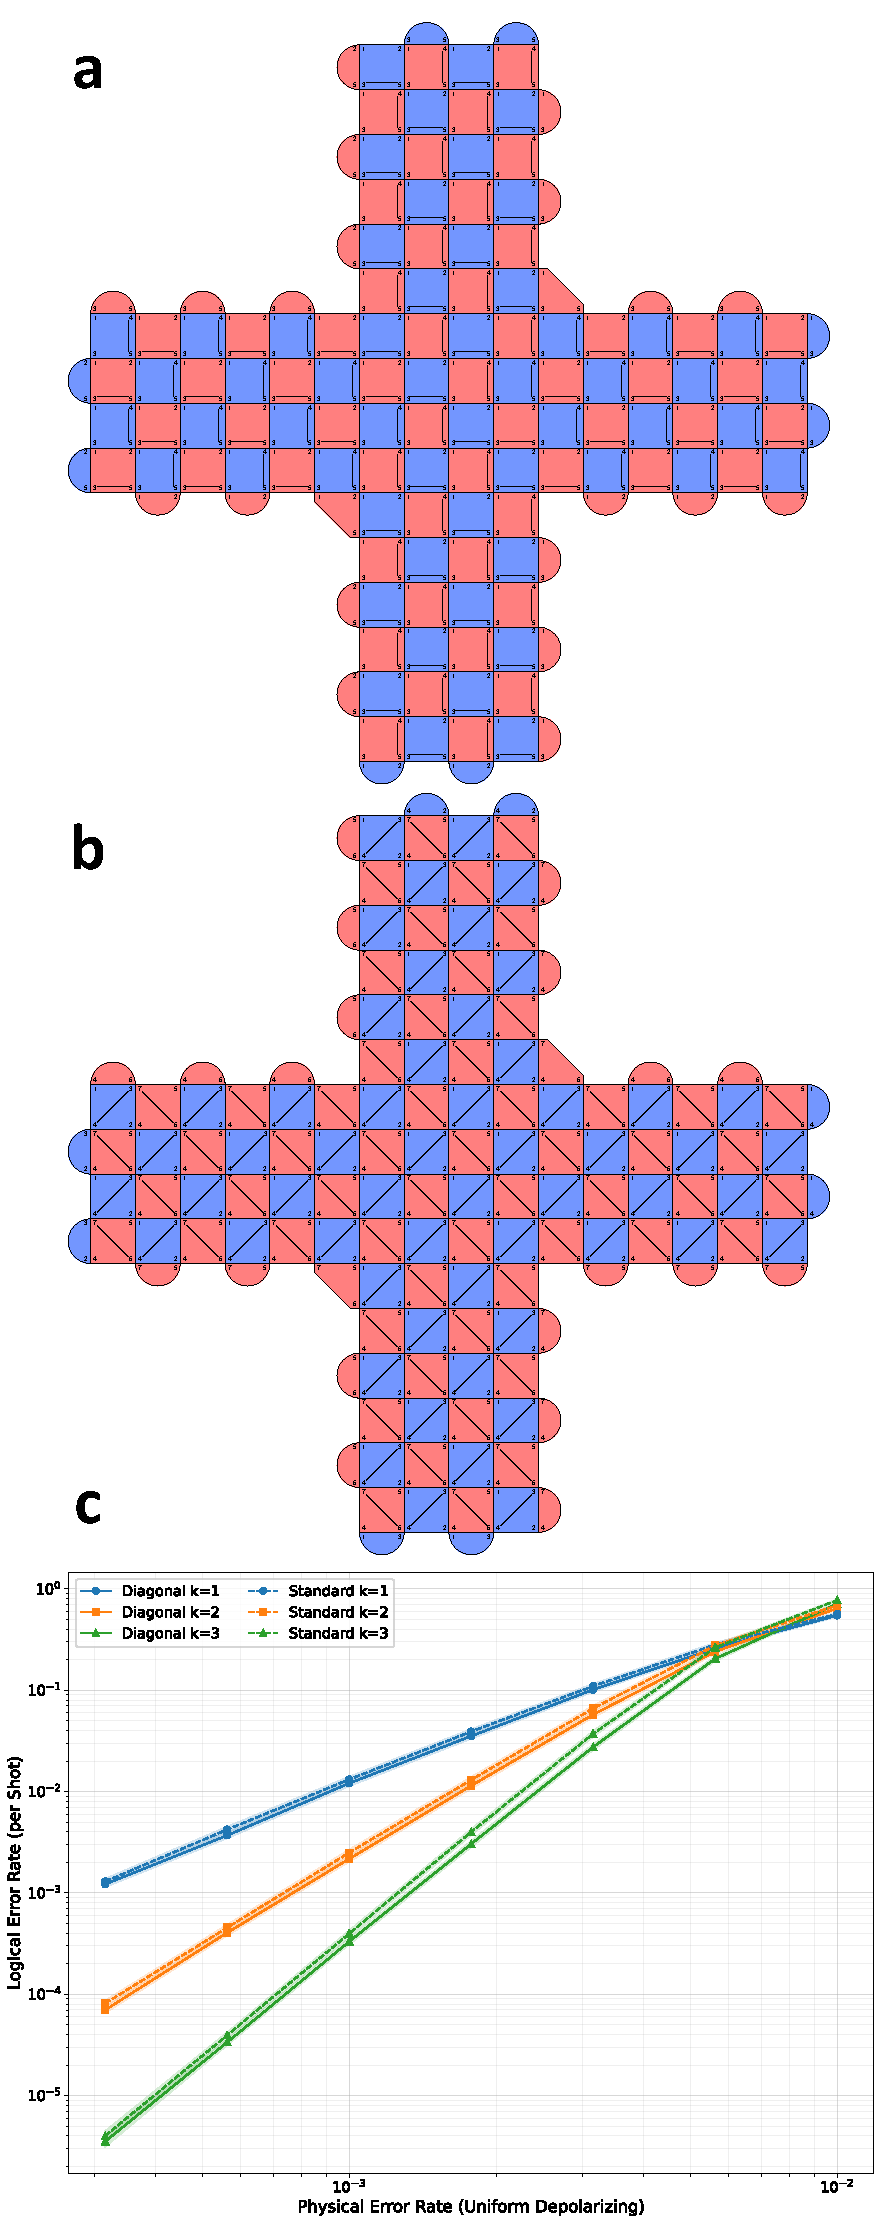
\includegraphics[width=\columnwidth]{x_junction.pdf}
\caption{
X-shaped spatial junction.
\textbf{(a)} Standard schedule requiring careful orientation planning at the four-way junction.
\textbf{(b)} Diagonal schedule with uniform circuits throughout.
\textbf{(c)} Logical error rate comparison showing the diagonal schedule (solid) slightly outperforming the standard schedule (dashed).
This improvement arises because the diagonal schedule enables a more compact period-4 circuit, while the standard schedule requires period-5 to avoid gate collisions at the junction.
}
\label{fig:x_junction}
\end{figure}

The X-junction is particularly challenging for traditional scheduling because plaquettes at the center of the junction have neighbors in all four directions, making it difficult to find an orientation that avoids all problematic hook error paths.

Panel (c) shows that the diagonal schedule actually achieves slightly lower logical error rates than the standard schedule for this geometry.
This improvement comes from the reduced circuit period: the diagonal schedule's global uniformity allows a period-4 circuit, while the standard schedule requires period-5 to accommodate different orientations in adjacent plaquettes without gate collisions.

\section{Spatial Hadamard}
\label{sec:hadamard}

The spatial Hadamard gate exchanges the X and Z logical operators of a surface code patch by rotating the patch geometry.
This operation involves stretched stabilizers at the interface between the original and rotated regions.

\begin{figure}
\centering
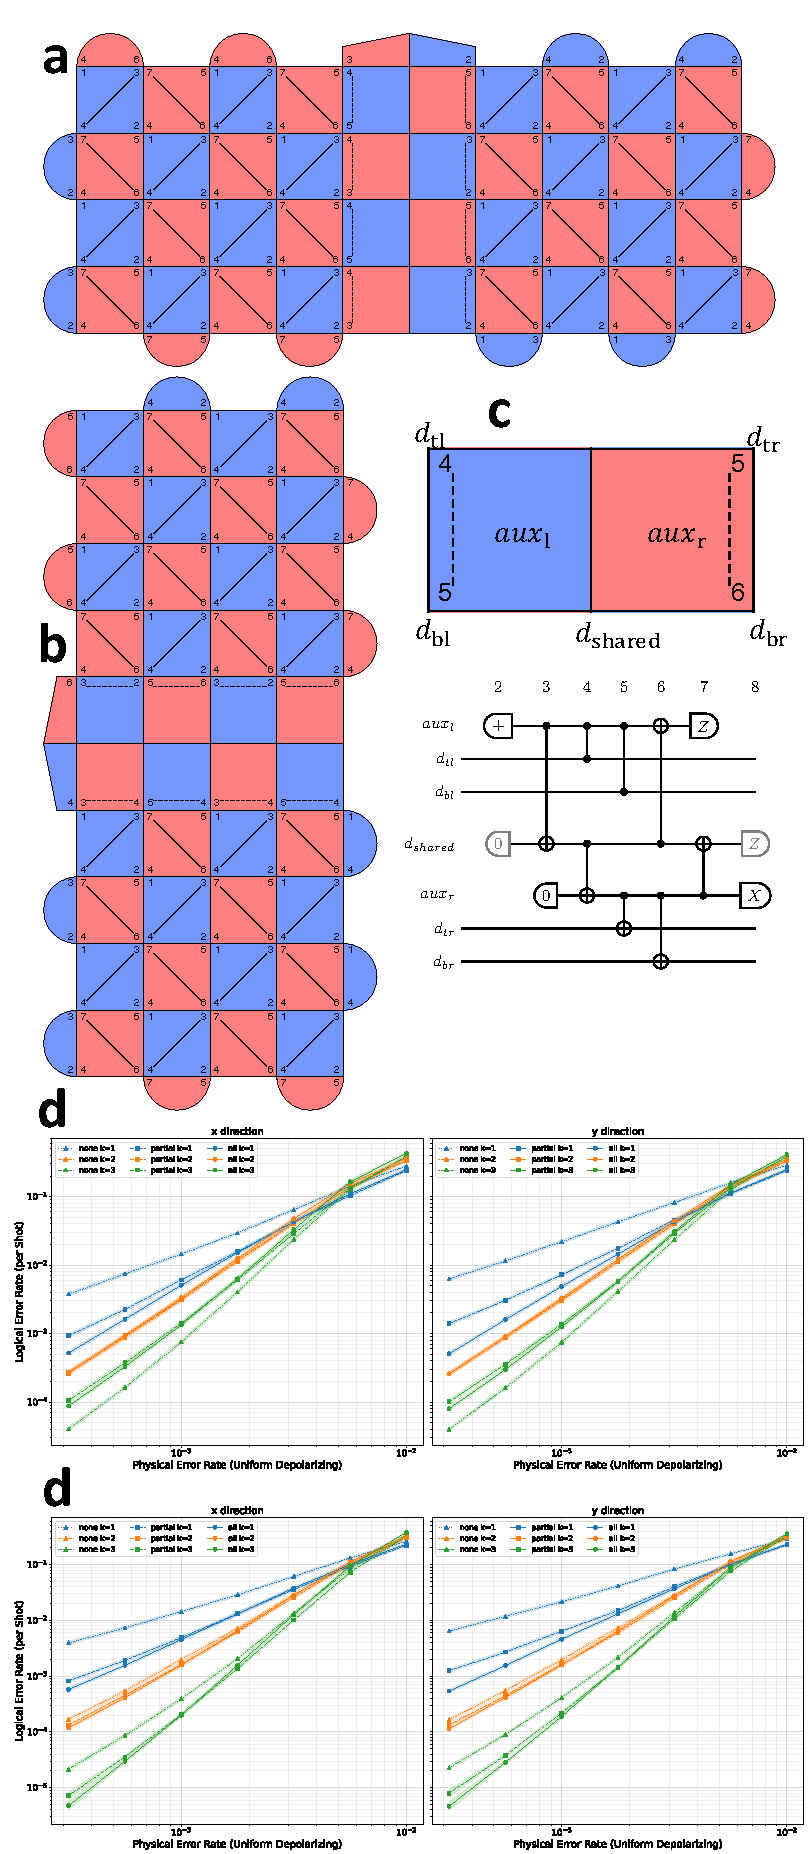
\includegraphics[width=\columnwidth]{hadamard.pdf}
\caption{
Spatial Hadamard gate with the diagonal schedule.
\textbf{(a)} Vertical spatial Hadamard showing the interface region with stretched stabilizers.
\textbf{(b)} Horizontal spatial Hadamard.
\textbf{(c)} Detailed view of the stretched stabilizer geometry and the corresponding syndrome extraction circuit.
Stretched stabilizers are prone to hook errors along their short direction.
Flag measurements (shown in circuit) detect these problematic hook errors without increasing circuit depth, as the flag measurement can occur in parallel with other operations.
\textbf{(d)} Logical error rate versus physical error rate using PyMatching decoder, with separate panels for horizontal (left) and vertical (right) Hadamard directions.
\textbf{(e)} Same benchmarks using correlated PyMatching, which can exploit the flag measurement information.
Some errors that would be matchable without flags become non-matchable when flag information is included, improving decoder performance.
}
\label{fig:hadamard}
\end{figure}

The stretched stabilizers at the Hadamard interface present a unique challenge.
These stabilizers span a rectangular rather than square region, making them particularly susceptible to hook errors along their short axis.
Such hook errors could create shortcuts for logical errors if not properly handled.

Our solution introduces flag measurements that detect when problematic hook errors occur on stretched stabilizers.
Crucially, these flag measurements come ``for free'' in terms of circuit depth---they can be performed in parallel with other operations in the syndrome extraction circuit.

When a flag triggers, it indicates that a hook error has occurred and the decoder should treat the situation accordingly.
With a correlated matching decoder that can use flag information, some errors that would otherwise be matchable become non-matchable, improving the decoder's ability to correctly identify error chains.

Panels (d) and (e) compare performance with standard PyMatching and correlated PyMatching decoders.
The correlated decoder shows improved performance, particularly at higher physical error rates, by exploiting the additional information provided by flag measurements.

\section{Patch Rotation}
\label{sec:rotation}

Patch rotation is another important lattice surgery primitive that reorients a surface code patch.
Figure~\ref{fig:rotation} shows the diagonal schedule implementation of a patch rotation circuit.

\begin{figure}
\centering
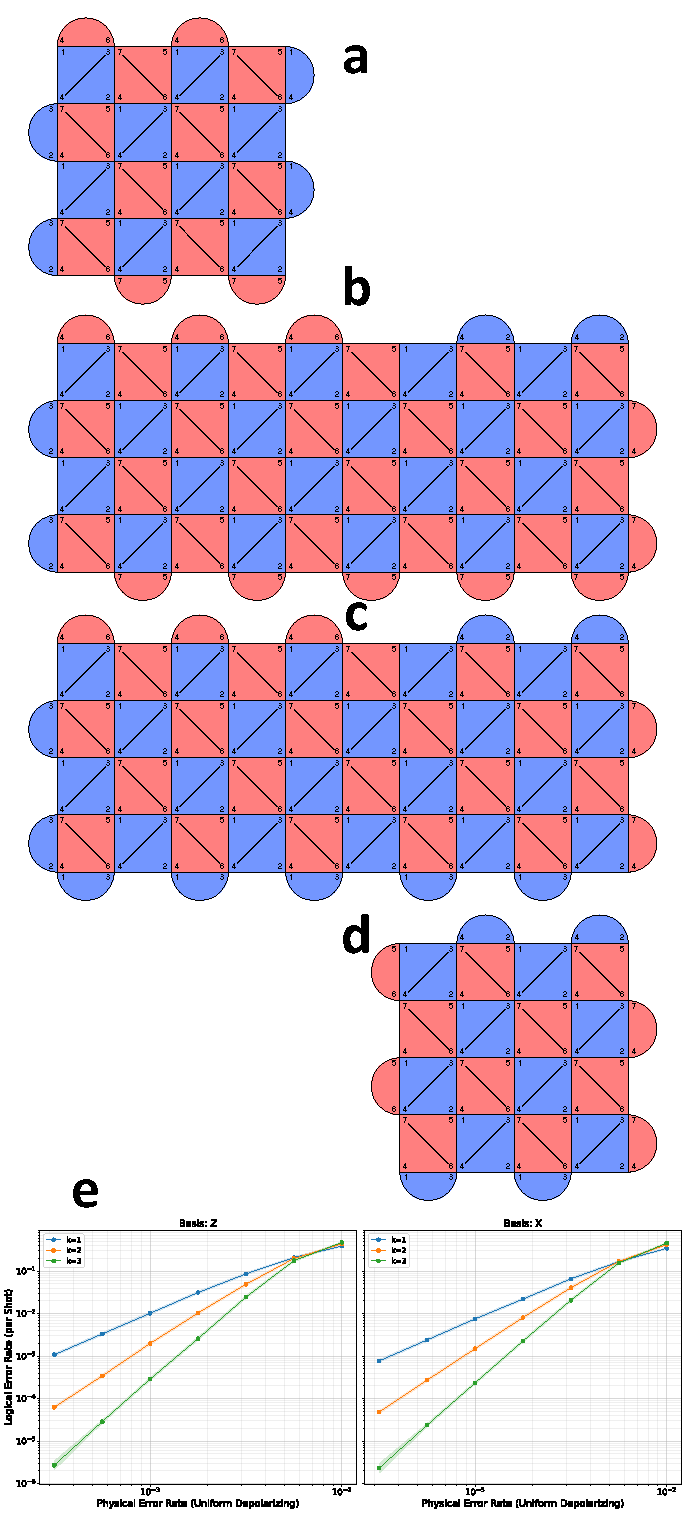
\includegraphics[width=\columnwidth]{rotation.pdf}
\caption{
Patch rotation with the diagonal schedule.
\textbf{(a)--(d)} Four time steps during the patch rotation circuit, showing how the patch geometry evolves.
The diagonal schedule maintains its uniform structure throughout the rotation.
\textbf{(e)} Logical error rate benchmarks for the X observable (left panel) and Z observable (right panel) during patch rotation.
Different colors indicate different code distances $d = 2k+1$.
}
\label{fig:rotation}
\end{figure}

The patch rotation involves a sequence of stabilizer modifications that gradually transform the patch orientation.
Throughout this process, the diagonal schedule maintains its uniform structure, with all X-type plaquettes using the same circuit and all Z-type plaquettes using their corresponding circuit.

Panel (e) shows the logical error rates for both X and Z observables during the rotation.
The diagonal schedule successfully preserves the code distance for both logical operators throughout the rotation process.

\section{Summary}
\label{sec:summary}

We have presented the diagonal schedule for surface code syndrome extraction, which addresses the limitations of traditional N-shaped and Z-shaped scheduling approaches.

The key advantages of the diagonal schedule are:
\begin{enumerate}
    \item \textbf{Hook error immunity}: Diagonal hook errors trigger four stabilizers and never reduce logical operator weights, regardless of boundary geometry.
    \item \textbf{Global uniformity}: All plaquettes of the same type use identical circuits, eliminating geometry-dependent schedule planning.
    \item \textbf{Compact period}: The uniform schedule enables period-4 operation on suitable hardware, compared to period-5 for mixed N/Z schedules.
    \item \textbf{Simplified construction}: Complex lattice surgery operations become straightforward to implement without careful hook error analysis.
\end{enumerate}

We demonstrated the diagonal schedule across a range of important use cases: memory experiments, L-junctions, X-junctions, spatial Hadamard gates, and patch rotations.
In all cases, the diagonal schedule achieves equivalent or better logical error rates compared to traditional approaches while significantly simplifying circuit construction.

For spatial Hadamard gates involving stretched stabilizers, we introduced flag measurements that detect problematic hook errors without increasing circuit depth.
These flags enable correlated decoders to achieve improved performance by making certain error patterns non-matchable.

Two additional cases of significant importance that are expected to benefit from the diagonal schedule are the yoked surface code~\cite{gidney2025yoked} and the crosshairs surface code~\cite{litinski2025crosshairs}.
Both constructions allow storing logical qubits more compactly for a given code distance by concatenating surface codes into outer codes with complex boundary structures.
The diagonal schedule's global uniformity and geometry-independent hook error handling make it particularly well-suited for these advanced architectures.

The diagonal schedule represents a practical improvement for surface code implementations, particularly for systems performing lattice surgery computations where varied boundary geometries would otherwise require complex schedule planning.
Its global uniformity and compact period make it an attractive choice for near-term fault-tolerant quantum computing systems.

All syndrome extraction circuits were constructed using the TQEC library~\cite{tqec2024} and simulated using Stim~\cite{gidney2021stim}.
Decoding was performed using PyMatching~\cite{higgott2023pymatching}.

\acknowledgments

We thank Ron Cohen, Shoham Jacobi, Peter-Jan H. S. Derks, Craig Gidney, Oscar Higgott, Adrien Suau, Yaar Vituri, Arabella Schelpe    for useful discussions.

\bibliography{references}

\end{document}
